% Канонический TikZ-рисунок варианта 02. Править только здесь.
\long\def\figStereoV02{%
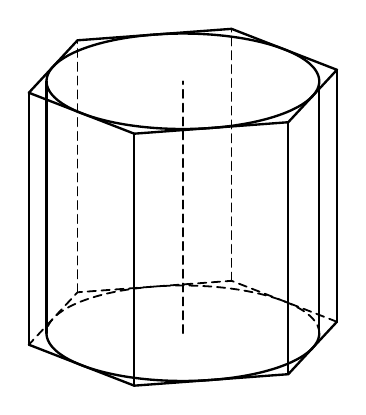
\begin{tikzpicture}[
    x={(1cm,0cm)},
    y={(0cm,0.35cm)},
    z={(0cm,1cm)},
    line cap=round,
    line join=round,
    visible/.style={line width=0.85pt},
    hidden/.style={line width=0.65pt,dashed,dash pattern=on 3pt off 2pt}
]

% =========================================================
% Параметры
% =========================================================

\def\a{2}      % сторона правильного шестиугольника
\def\H{3.2}    % высота призмы
\def\phi{12}   % угол поворота основания

% Радиус вписанной окружности правильного шестиугольника
\pgfmathsetmacro{\r}{sqrt(3)*\a/2}

% =========================================================
% Вершины нижнего основания
% =========================================================

\coordinate (A0) at ({\a*cos(\phi)},      {\a*sin(\phi)},      0);
\coordinate (A1) at ({\a*cos(60+\phi)},   {\a*sin(60+\phi)},   0);
\coordinate (A2) at ({\a*cos(120+\phi)},  {\a*sin(120+\phi)},  0);
\coordinate (A3) at ({\a*cos(180+\phi)},  {\a*sin(180+\phi)},  0);
\coordinate (A4) at ({\a*cos(240+\phi)},  {\a*sin(240+\phi)},  0);
\coordinate (A5) at ({\a*cos(300+\phi)},  {\a*sin(300+\phi)},  0);

% =========================================================
% Вершины верхнего основания
% =========================================================

\coordinate (B0) at ({\a*cos(\phi)},      {\a*sin(\phi)},      \H);
\coordinate (B1) at ({\a*cos(60+\phi)},   {\a*sin(60+\phi)},   \H);
\coordinate (B2) at ({\a*cos(120+\phi)},  {\a*sin(120+\phi)},  \H);
\coordinate (B3) at ({\a*cos(180+\phi)},  {\a*sin(180+\phi)},  \H);
\coordinate (B4) at ({\a*cos(240+\phi)},  {\a*sin(240+\phi)},  \H);
\coordinate (B5) at ({\a*cos(300+\phi)},  {\a*sin(300+\phi)},  \H);

% =========================================================
% Невидимые части нижнего основания призмы
% =========================================================

\draw[hidden] (A0)--(A1)--(A2)--(A3);

% =========================================================
% Невидимые вертикальные рёбра
% =========================================================

\draw[hidden] (A1)--(B1);
\draw[hidden] (A2)--(B2);

% =========================================================
% Невидимая задняя половина нижней окружности цилиндра
% =========================================================

\draw[hidden]
    plot[domain=0:180,samples=100,variable=\t]
    ({\r*cos(\t)},{\r*sin(\t)},0);

% =========================================================
% Ось цилиндра
% =========================================================

\draw[hidden] (0,0,0)--(0,0,\H);

% =========================================================
% Видимые вертикальные рёбра призмы
% =========================================================

\draw[visible] (A0)--(B0);
\draw[visible] (A3)--(B3);
\draw[visible] (A4)--(B4);
\draw[visible] (A5)--(B5);

% =========================================================
% Видимая передняя часть нижнего основания призмы
% =========================================================

\draw[visible] (A3)--(A4)--(A5)--(A0);

% =========================================================
% Образующие цилиндра
% =========================================================

\draw[visible] (-\r,0,0)--(-\r,0,\H);
\draw[visible] ( \r,0,0)--( \r,0,\H);

% =========================================================
% Видимая передняя половина нижней окружности цилиндра
% =========================================================

\draw[visible]
    plot[domain=180:360,samples=100,variable=\t]
    ({\r*cos(\t)},{\r*sin(\t)},0);

% =========================================================
% Верхнее основание призмы
% =========================================================

\draw[visible] (B0)--(B1)--(B2)--(B3)--(B4)--(B5)--cycle;

% =========================================================
% Верхняя окружность цилиндра
% =========================================================

\draw[visible]
    plot[domain=0:360,samples=160,variable=\t]
    ({\r*cos(\t)},{\r*sin(\t)},\H);

\end{tikzpicture}
}
